\documentclass[12pt]{article}%% 12-point Times New Roman font
\usepackage{geometry}
\usepackage{booktabs}
\usepackage{multirow}
\usepackage{array}
\usepackage{setspace}
\usepackage[linesnumbered,ruled,lined]{algorithm2e}
\usepackage{amsmath,amssymb}
\usepackage{graphicx}
\usepackage{subfigure}
\usepackage{fancybox}
\usepackage[bottom]{footmisc}
\usepackage{fancyhdr}
\usepackage{float}
\usepackage{listings}
\usepackage{lastpage}
\usepackage{fontspec}% 便于修改字体
\usepackage{xcolor}
\usepackage{hyperref}
%%%%%%%%%%%%%%%%%%%%%%%%%%%%跟新字体%%%%%%%%%%%%%%%%%%%%%%%%%%%%%%%%%%
\usepackage{newtxmath} % 数学字体
\usepackage{newtxtext}%\usepackage{palatino}
\usepackage{amsmath,amssymb}
\usepackage{indentfirst}	%开头空两个
%%%%%%%%%%%%%%%%%%%%%%%%%%%%%%%%%%%%%%%%%%%%%%%%%%%%%%%%%%%%%%%%%%%%%
\hypersetup{
	unicode={true},pdfstartview={FitH},pdfborder={0 0 0},
	colorlinks,linkcolor=black,citecolor=black,hyperindex,plainpages=false,
}
\hypersetup{
	colorlinks=true,
	linkcolor=black
}
% style: page layout
\setlength{\headheight}{17pt}
\setlength{\headsep}{20pt}
\setlength{\footskip}{30pt}
\addtolength{\textheight}{3\baselineskip}
\newtheorem{definition}{{definition}}
\newcounter{numdefinition}
\renewenvironment{definition}[1]
{\noindent\stepcounter{numdefinition}
\slshape Definition \arabic{numdefinition} \textsf{#1 :}
	\begin{quote}\small\itshape}
	{\end{quote}}
\fancypagestyle{plain}
{\fancyhf{}
	\setlength{\headheight}{0pt}\setlength{\headsep}{0pt}
	\setlength{\voffset}{-70pt}\setlength{\oddsidemargin}{0pt}}
\graphicspath{{pic/}}

%=============================新的命令=================================
\newcommand{\dd}{\ensuremath{\,\mathrm{d}}}
\newcommand{\upcite}[1]{\textsuperscript{\cite{#1}}}
\newcommand{\headset}{{\Large\the\year}\\MCM/ICM\\Summary Sheet}
\newcommand{\vw}{\frac{v_i}{\omega_i}}
\renewcommand{\thefootnote}{\arabic{footnote}}

%===========================每一页的页注===============================
\pagestyle{fancy} 
%\rhead{page \thepage\ of \pageref{LastPage}}	%注意设置到附录就行!!
%\chead{} \lhead{Team \footnotesize{\#} 2015970} \lfoot{}	%#为题号,9999为队伍编号
%\cfoot{\thepage}
%\rfoot{}
\renewcommand{\headrulewidth}{0.4pt}
%%%%%%%%%%%%%%%%%%%%%%%%%%%%中文宏包%%%%%%%%%%%%%%%%%%%%%%%%%%%%%%%%%%%
%\usepackage[UTF8]{ctex}
%%%%%%%%%%%%%%%%%%%%%%%%%%用了后会缩水%%%%%%%%%%%%%%%%%%%%%%%%%%%%%%%%%


\begin{document}
\newpage
\thispagestyle{empty}
\newgeometry{top=3cm, left=3.5cm, right=3.5cm}
\vspace*{-5pc}%
\setmainfont{Times New Roman}

\begin{center}
	\begingroup
	\setlength{\parindent}{0pt}
	\begin{minipage}[t]{0.33\linewidth}
		\bfseries\centering%
		Problem Chosen\\[0.7pc]
		{\Huge\textbf{\textcolor{red}{C}}}\\[2.8pc]
	\end{minipage}%
	\begin{minipage}[t]{0.33\linewidth}
		\centering%
		\textbf{\headset}%
	\end{minipage}%
	\begin{minipage}[t]{0.33\linewidth}
		\centering\bfseries%
		Team Control Number\\[0.7pc]
		{\Huge\textbf{\textcolor{red}{2015970}}}\\[2.8pc]
	\end{minipage}\par
	\vskip 10pt%
	\rule{\linewidth}{1.5pt}\par
	\endgroup
	\vskip 10pt%
\end{center}
%%%%%%%%%%%%%%%%%%%%%%%%%%%%%%%%%Title%%%%%%%%%%%%%%%%%%%%%%%%%%%%%%%%%%%%
\begin{center}
	\vspace{10pt}
	{\normalfont \LARGE \textbf{ Title Title Title} }\par
	\par		%换行=\\
	\vspace{7pt}
	\noindent
	{\textbf{Summary}}
\end{center}


%%%%%%%%%%%%%%%%%%%%%%%%%%%%%%%Abstract%%%%%%%%%%%%%%%%%%%%%%%%%%%%%%%%%%%
 In this paper, we offer mathematic descriptions of this topic and attempt to figure out optimal strategy on different emphasis-distance and gliding time.
~\\

 In this paper, we offer mathematic descriptions of this topic and attempt to figure out optimal strategy on different emphasis-distance and gliding time.
 ~\\
 
  In this paper, we offer mathematic descriptions of this topic and attempt to figure out optimal strategy on different emphasis-distance and gliding time.

\vspace{7pt}
\textbf{keyword}: Runge-Kutta; Aerodynamics


%%%%%%%%%%%%%%%%%%%%%%%%%%%%%%%%%%%%%%%%%%%%%%%%%%%%%%%%%%%%%%%%%%%%%%%

\newpage
\thispagestyle{empty}
{\large \textbf{Dear Market Director,}}

As consultants of Sunshine Company, it is our obligation to assist you in data analysis regarding the relationship and connections of 3Rs (Ratings, Reviews and Ratings of Reviews) of online shopping platforms. We are writing this letter to report our latest findings.

We design Sentiment Prediction Model to investigate the correlation between ratings and reviews. As ratings denote the quality of products in a general sense, the ratings of reviews signify whether a review can represent the experience of a common customer. To address the problem of variety of reviews, we conduct two operations, stemming and merging, to standardize the input. Two false scenarios, five stars on products of poor quality and one star mistakenly marked on genuine reviews, are 95\% filtered out by Logistic Regression. After an in-depth study of sentiment prediction, we conclude that certain descriptors of quality are remarkably bound up withs specific ratings, which is commensurate to our common sense.

In view of already available sentimental scores, we establish Dynamic Time Warping Model to research the connections between particular rating levels and the amount of reviews. The difference between the warped signals and original signals are trivial, which is the mathematical proof that specific rating levels are more likely to incite more reviews. We can also induce that among three products, pacifiers cling to corresponding reviews to a greater extent.

(Results of 2.a, remains to be discussed) Additionally, we develop Association Rule Analysis to examine the text-base and time-based measures that represent the soundness of the enterprise. We use gradient descent decision-making tree to filter the word vectors. This method not only accelerates the algorithm, but it also help us gain parameters shown in Appendix \ref{Appendices}.

In conclusion, our model successfully explains the correlations between ratings and reviews. Because the models and evaluation approaches are data-propelled, its applications in future online marketing problems, especially in customer services, are promising.

Integrating the analysis above, we propose following strategies for your consideration:

\begin{itemize}
	\item[1.]\textbf{Trace the source of quality texts.(这里附上Appendix名字)} Synthesizing customer advice can be tough. The list regarding quality descriptors and coefficient can represent the importance level and similarities of different customers’ voice. We recommend you retrieve the reasons why customers leave their comments by locating the source of customers which is feasible owing to trading recordings. Refined feedback chart in accordance with coefficient (importance) can better facilitate the improvements of your company.
	\item[2.]\textbf{Treat three products with different perspectives.} We find that in the list of coefficients concerning three products, though the top positive coefficients are almost identical, the absolute value of negative coefficient of pacifier is saliently greater. The compatibility of our parameter indicates that for the sake of long-term soundness of your enterprise, more attention and subtlety are required in ameliorating the quality of pacifier. 
	\item[3.]\textbf{View text-based and time-based measures in time-series patterns.} Views of customers can alter in time. We deem it plausible to conduct our operations in time-series patterns for the generality of business practices.
\end{itemize}

We have a strong belief that our model can effectively enhance the efficiency of online customer service and provides an appropriate as well as feasible way to best improve the business performance of your products.



\thispagestyle{empty}

%%%%%%%%%%%%%%%%%%%%%%%%%%%%%%%目录%%%%%%%%%%%%%%%%%%%%%%%%%%%%%%%%%%%%%%
\newpage
\thispagestyle{empty}
\tableofcontents   
\setcounter{page}{0}                                               
\newpage      

%%%%%%%%%%%%%%%%%%%%%%%%%%%%%%%正文设置%%%%%%%%%%%%%%%%%%%%%%%%%%%%%%%%%%%%%%%%
%\large					%%%%%%%该方法把字体跟中文的一样大了!!!!可以放到摘要前
\fontsize{13}{12.5}\selectfont
\setmainfont{TeX Gyre Pagella}    
\newgeometry{top=3cm, left=3.5cm, right=3.5cm}
\pagestyle{fancy} 
\rhead{page \thepage\ of 20}	%注意设置到附录就行!!
\chead{} \lhead{Team \footnotesize{\#} 2015970} \lfoot{}	%#为题号,9999为队伍编号
\cfoot{\thepage}
\rfoot{}
%%%%%%%%%%%%%%%%%%%%%%%%%%%%%%%正文开始%%%%%%%%%%%%%%%%%%%%%%%%%%%%%%%%%%%%%%

\section{Introduction}	
\subsection{Background}
Platforms for the public to swap purchase experiences are designated to spur the proceedings of trade process. Rating systems, especially in terms of reviews, are of significance in opinion alteration for prudent developers.
	
From the perspective of contributors, customers are inclined to go about browsing previous feedback, i.e. reviews prior to their purchases. Helpfulness ratings serve as pre-perceived expertise during other customers’ purchase decisions or simply become a practice of values interaction \footnote{\quad https://www.amazon.com/gp/help/customer/display.html?nodeId=G3UA5WC5S5UUKB5G}.

On the other hand, customer-based texts can constitute a recommendation in a recommender-rich environment like Amazon. No recommender system can be $100\%$ correct or produce systematically novel and haphazard results\cite{bib:1, bib:2} . To some extent, ratings of products and of reviews are dominant factors presented on a public platform without voir dire, which might offer misleading information about the merchant.

 Consequently, crucial analysis in recessive factors like selection of reviews that possess the most valid contents allows e-commerce companies to make improvements and adjustments to proffer products with high quality and subtlety\cite{amsu}.
 
We place great emphasis on the correlation between customer reviews, ratings and the ratings of reviews to determine period-choice sales patterns and help key features of three products to percolate down the industry for Sunshine company.


%------------------------------普通图片-----------------------------------------
\begin{figure}[H]
	\centering
	
\includegraphics[width=.7\textwidth]{pic/protect.jpg}%.4代表宽度大小正常为1
	\caption{Mapping description of the relationship between Amazon reviews and users via Visio.}\label{Suzanne}%caption里面是题目,label为标签,\ref引用
\end{figure}



\subsection{Related Works}

Danescu and Kossinets \cite{232}took Amazon as an example to assess how opinions are evaluated by members of an online community in a large scale. They found out that a review’s helpfulness depends not only on the content, but also on the relation of its score to other scores. The result resonates with the findings by Leino et al.\cite{236}, which underscore the significance of a recommender system as a whole. Direct recommendations proffer clients a closer scrutiny of their preferences.

Nicolau \cite{233} noted that extreme ratings (positive or negative) coexist with polarized sentiments with asymmetrical effects. A new dimension of reviews called “trustfulness” was developed by Kokkodis \cite{234} to construct models to rank customers, which later to be proved thought-provoking in future application scenarios like whether to put the review contains information exposed only to buyers. 

Models above have presented overwhelming standpoints on the impact of local features or recommender system. However, for e-commerce companies like Amazon and e-Bay, comprehensive trade strategies entail a deliberate combination of measures to ensure enterprise’s soundness.

We adopt ??? to ascertain the relationship of reviews and ratings of 1st and 2nd order. In our model, a series of word vectors are generated from reviews to execute attention mechanism for ideal output to separate reviews. We use a data set originated from Amazon to test our theories to prove efficacy and robustness.
	

\subsection{Our Works(会做调整))}
The main contributions of this paper are as follows:
%1我们找出了specific descriptors strongly associated with the rating levels,依据评价和分数制定了数据度量,并基于此选择出了最有价值的信息。
\begin{itemize} 
	\item [1.] We utilize ??? to quarry the descriptors that are strongly associated with the rating levels and turn them into sentimental scores to serve as text-based measures. 
	%找出反应评星的词,然后变成情感分
	\item [2.] In accordance with the ratings-based patterns and text-based approaches, we rate reliability of each review in ??? to identify the most track-worthy one.      
	%找出最值得track的review-----------a
	\item [3.] We design the time-based measures that can reflect the fluctuation of the product’s reputation. 
	%名声和时间策略的关系------------b
	\item [4.] We adopted Association Rule Analysis(-AR) to find the combinations of text-based measures and ratings-based measures that can reveal the success or failure of the products.
	%寻找反应产品好坏的时间和评星策略--------------c
	\item [5 .]We used the Dynamic Time Warping(DTW) is  to verify whether the specific star ratings incite more reviews with the same sentiment.
	%回答:是否特定的评星在同样的感情下引起更多的评论---------------d
	%\item [5.]Based on the measures identified in this paper, we propose the best online sales strategy to the Marketing Director.
\end{itemize}

\section{Fundamental Assumptions}
\begin{enumerate}
	\item  To guarantee our modeling process is reasonable, we assume most of the reviews are rational.  
\end{enumerate}

\section{Nomenclature}

	\begin{table}[H]
	\label{biao} \centering
	\begin{tabular}{cc}
		\toprule[1.5pt]
		\multicolumn{1}{m{3cm}}{\centering Symbols} & \multicolumn{1}{m{10cm}}{\centering Definitions} \\
		\midrule[1pt]
		$x$	 &  distance from infinitesimal $dx$ to $x$ axis\\
		\bottomrule[1.5pt]
	\end{tabular}
\end{table}


%%%%%%%%%%%%%%%%%%%%%%%%%%%%%%%预备工作%%%%%%%%%%%%%%%%%%%%%%%%%%%%%%%%%%%%%%

\section{Rating-based Measure}
Before identifying the rating-based measure, the rating distribution of the three kinds of products can be visualized as below 
%As shown in Figure \ref{scosssre}, the possible values of star ratings are integers from 1 to 5. We define the reviews with Score 1,2 as Negative reviews and Score 4,5 to be Positive reviews. The Neutral reviews with Score 3 are removed, which merely occupy a small part of the database.


\begin{figure}[H]
	\centering
	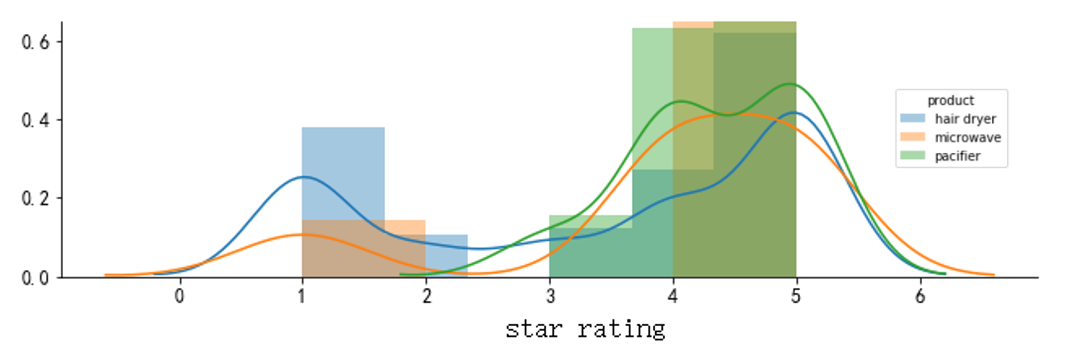
\includegraphics[width=1\textwidth]{score.png}%.4代表宽度大小正常为1
	\caption{The 'star\_rating' with the distribution of 'vine'	}\label{scosssre}%caption里面是题目,label为标签,\ref引用
\end{figure}

为了衡量rating的quantitative and qualitative patterns,我们采用以下常见的度量标准,计算结果如表\ref{biasssssssso}所示.

\textbf{Skewness -} 偏度是统计数据分布偏斜方向和程度的度量,是统计数据分布非对称程度的数字特征,其计算方式为$\text { Skew }(X)=E\left[\left(\frac{X-\mu}{\sigma}\right)^{3}\right]=\frac{k_{3}}{\sigma^{3}}=\frac{k_{3}}{k_{2}^{3 / 2}}
$

\textbf{Net Promoters Score -} 
As a gauge that represents how the enterprise and employees treat customers, NPS signals the possibility that users recommend products and services to their colleagues and friends. In this sense, customers are classified as recommenders, passives and detractors. NPS helps us evaluate customer satisfaction and loyalty\cite{nsp}. NPS is defined as
%NPS(Net Promoters Score) 是现有用户向其他人推荐你的产品和服务的可能性指数。是一种用来测量企业及员工如何对待客户的度量指标。在这一度量内,客户被划分为三大种类:推荐者、被动者和贬损者。也就是客户是否愿意将公司或产品推荐给朋友或同事。通过NPS helps us evaluate customer satisfaction and loyalty\cite{nsp}, 其计算方式如下:
\begin{gather}
NPS = (Promoters - Detractors)/Total ratings * 100
\end{gather}
Where the reviews with rating 1,2 are regarded as Detractors while the ones with Rating 3 and Rating 4,5 are Passive and Promoters respectly.

\begin{table}[H]
	\centering
	\caption{Inciting rate of the best-sell product.}	
	\setstretch{1.3}  %设置表的行间距
	\begin{tabular}{cccc}
		\toprule[1.5pt]
		\multicolumn{1}{m{7cm}}{\centering Product title} & \multicolumn{1}{m{2cm}}{\centering Average}&
		\multicolumn{1}{m{2cm}}{\centering Skewness} &
		\multicolumn{1}{m{2cm}}{\centering NPS} \\
		\midrule[1pt]
		andis fold-n-go ionic hair dryer &4.5129&-1.51&73.66\\
		pearl ceramic hair dryer     & 4.6092&-1.33&75.55\\
		watt tourmaline ceramic hair dryer          &4.6252&-1.54&73.41\\
		\midrule[1pt]
		cu.ft. countertop microwave          &4.4476&-0.98&71.54\\
		wmc20005yw  countertop microwave          &3.8654&-1.41&62.47\\
		sharp microwave drawer oven        &3.9240&-1.31&67.58\\
		\midrule[1pt]
		free contemporary freeflow pacifier        &3.5277&-2.58&57.54\\
		free soothie pacifier       &4.2666&-2.69&71.15\\
		wubbanub infant pacifier&3.9115&-1.99&64.48\\
		\bottomrule[1.6pt]
	\end{tabular}\label{biasssssssso}
\end{table}


\section{Text-based Measure }
To quantify the text information in reviews and identify the text-based measures, we execute sentimental analysis to the reviews in this phase. Based on the measures, we could gain the specific quality descriptors that are strongly associated with rating levels.
\subsection{Text preprocessing}
Text datas should be cleaned and encoded into numerical values before machine learning models. This process of data cleaning and encoding is defined as Text Preprocessing.

\subsubsection{Data Cleaning}
	We define the reviews with Score 1,2 as Negative reviews and Score 4,5 to be Positive reviews. The Neutral reviews with Score 3 are removed, which merely occupy a small part of the database. Then the word vectors\cite{BOW} are gained after converting all the words to lowercase and removing punctuations. The we utilize the Stemming and Stopwords strategy to simplify the word vectors.
	%If we see the 'star\_rating' column, it has values 1,2,3,4,5. We consider 1, 2 as Negative reviews and 4, 5 as Positive reviews. For Score = 3 we will consider it as Neutral review and lets delete the rows that are neutral, so that we can predict either Positive or Negative. Then converting all words to lowercase and removing punctuations and html tags if any.
	



	\textbf{Stemming -} Transforming the words into their base words or stem words. This reduces the vector dimension. For instance, we merge homologous words like \textit{'efficiently', 'efficient'}  into their stem word \textit{'effect'}.
	
	\textbf{Stopwords -} Filtering words without actual semantemes like 'This microwave is so efficiently' become 'microwave', 'efficiently', then stopwords are removed.
	%that even if they are removed the sentiment of the sentence dosent change like  \footnote{. Ex - \textit{'This microwave is so efficiently'} become \textit{'microwave', 'efficiently'}, then stopwords are removed.}.


\subsubsection{Encoding}
	
    Raw text data should be converted into numerical vectors that can be recognized in machine learning. Thus, we adopt the popular encoding techniques as follows :

\begin{itemize} 
	\item  \textbf{Bag of Words \cite{BOW, BOW2}:} Bag of Words is to compute the frequency of the appearing times of each word. 
	\item  \textbf{TF-IDF \cite{TF} :} Term Frequency - Inverse Document Frequency guarantees that the less important but given to the most frequent words are also considered as less frequent words.
	
	\item  \textbf{Word2Vec \cite{word,word2,word3}:} Word2Vec actually draws the semantic meaning of the words and their relationships between other words. It extracts all the internal relationships between the words and turn the word into a vector form.

\end{itemize}
We utilize t-distributed Stochastic Neighborhood Embedding\cite{t} to visualize the high-dimension word vectors to be 2-dimension surface as Figure \ref{fig}.
%------------------------------一行两张图片--------------------------------------
\begin{figure}[H]
	\centering
	\subfigure[TSNE for TF-IDF]{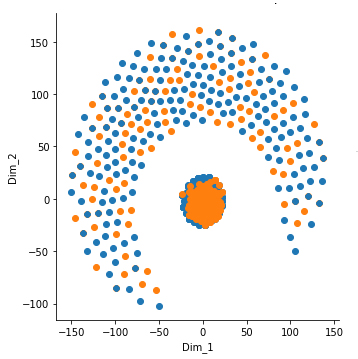
\includegraphics[height=7cm,width=7cm]{1.png}}
	\subfigure[TSNE for Word2Vec]{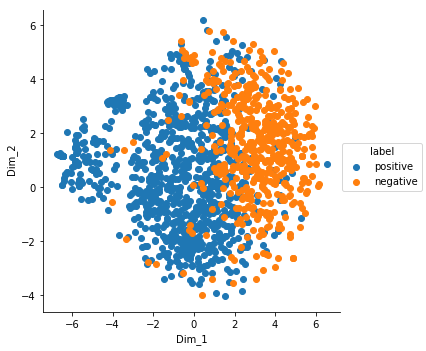
\includegraphics[height=7cm,width=7cm]{12.png}}
	\caption{ Vectors that perform well in classification.}
	\label{fig}
\end{figure}

Each plot in Figure \ref{fig} can represented a review in the dataset. The color of plot would be blue when the review is positive, while it would be orange as the review is nagetive. As the positive and negative plots can be separated in general, one could expect the TF-IDF and Word2Vec are able to separate the class labels in our dataset. Thus, we merge the word vectors in the two model into each other to gain the text feature.  

\subsection{Sentimental Analysis}
Before computing the sentimental rating for the each review, we would determine which words that are strongly associated with rating levels and draw the sentimental rating of this words based on the text feature yeilded in text preprocessing stage. Then the text-based measure can be gained by summing up the sentimental ratings of the words in each review. 
%The purpose of this phase is to establish a prediction model where we are able to predict whether a recommendation is positive or negative. In this analysis, we only focus on the positive/negative sentiment of the recommendation instead of concentrating on the Score. 

\subsubsection{Logistic Regression}
We adopt Logistic Regression to execute the binary classification for each review. The core model can be give as
%Logistic Regression model was designed to solve the binary classification problem\cite{lg}. Although its name includes the word regression, it merely implicitly operates a regression in its linear part. The ultimate goal is to solve the dichotomy problem. Its model is as follows:
\begin{gather}
y=\frac{1}{1+e^{-\left(w^{T} x+b\right)}}
\end{gather}
We apply the gradient descent algorithm and define the loss function as $L=-[y \log \hat{y}+(1-y) \log (1-\hat{y})]$, then we compare the predictions with the Bayesian algorithm \cite{bbb} as below

	\begin{figure}[H]
	\centering
	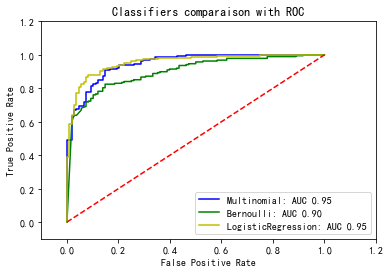
\includegraphics[width=0.8\textwidth]{111.png}%.4代表宽度大小正常为1
	\caption{The ROC curve for different algorithms.}\label{llll}%caption里面是题目,label为标签,\ref引用
\end{figure}

%以hair\_dryer为例,我们能看到Accuracy is around 95.9\%,并且前Top 10 negative/positive词如表\ref{biasso}所示.  However we notice that some of those significant coefficients are not meaningful, e.g. 'junk'.
 Figure \ref{llll} reveals that Accuracy is around 95.9\%. Top 10 negative/positive words are listed in Table \ref{biasso}. The coefficient reflect the confidence to result, which are positive correlation to the classification accuracy when the word is identified as positive word but nagetive correlation when negetive. As all $ \left | coefficient \right |>1 $, the classification result can be deemed to be reliable.

%以hair\_dryer为例,我们能看到Accuracy is around 95.9\%,并且前Top 10 negative/positive词如表\ref{biasso}所示.  However we notice that some of those significant coefficients are not meaningful, e.g. 'junk'.

\begin{table}[H]
	\centering
	\caption{Logistic regression model on word count}	
	\setstretch{1.3}  %设置表的行间距
	\begin{tabular}{cccc}
		\toprule[1.5pt]
		\multicolumn{1}{m{3cm}}{\centering positive word} & \multicolumn{1}{m{3cm}}{\centering coefficient}&
		\multicolumn{1}{m{3cm}}{\centering negative word}&
		\multicolumn{1}{m{3cm}}{\centering coefficient} \\
		\midrule[1pt]
		love     	 & 2.020178 & stop   &-2.655619\\
		excel     & 1.967720 &disappoint    &-1.985671\\
		perfect     &1.775876&wast    &-1.935428\\
		great          &1.775876&junk        &-1.736096\\
		 nice     &1.727514& suck    &-1.695555\\
		definit          & 1.698679& fail    &-1.679773\\
		awesom          &1.633642&defect        &-1.612045\\
		best        &1.612823&poor      &-1.595778\\
amaz        &1.403347&worst       &-1.464123\\
fast       &1.259788&broke          &-1.567801\\
		\bottomrule[1.6pt]
	\end{tabular}\label{biasso}
\end{table}
The WordNetLemmatizer from NLTK\footnote{\quad Library from http://www.nltk.org/nltk\_data/} can be applied to determine the morphemes by gathering word class. Horizontally examining 2-gram and 3-gram, one can analyse ratings of different products and extract identical characteristics of the contexts. Focusing on popular single \textbf{adjective} rating words, one can gain phrases that occur more than benchmarks of reviews. We take the database of hair dryer as an example, the result could be showed in the cloud map as follow

%In a ispecific hair\_dryer situaton, we analyse each rating level.By means of  WordNetLemmatizer from NLTK\footnote{. http://www.nltk.org/nltk\_data/}, morphemes can be determined by gathering word class. Horizontally looking at 2-gram and 3-gram, we analyse ratings of different products and extract identical characteristics of the contexts. Then we focus on popular single \textbf{adjective} rating words. We modify the function to return only phrases that occur more than benchmarks of reviews. We display the results in the cloud map.
%同样以hair\_dryer为例,对每个星级分别进行分析,利用NLTK\footnote{. http://www.nltk.org/nltk\_data/}的WordNetLemmatizer可以用gathering的词类确定词元。when look at 2-gram and 3-gram together, 我们通过不同用户ID对于不同的产品对打分情况进行分析,并提取文本中的同特征。 Then we focus on popular single \textbf{adjective} word people used for different score and  modify the function that return only phrase occurs more than benchmark of someone reviews. 可以得到结果可以用云图绘制出来:
\begin{figure}[H]
	\centering
	\subfigure[Negitive words]{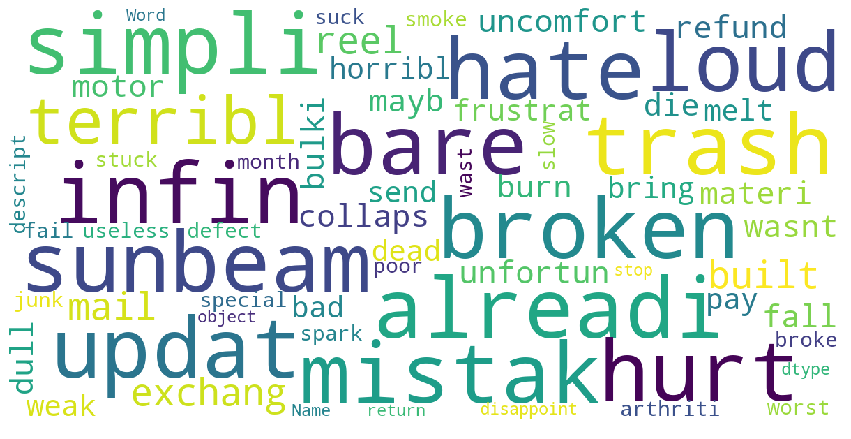
\includegraphics[height=7cm,width=14cm]{neg.png}}
	
	\subfigure[Postive words]{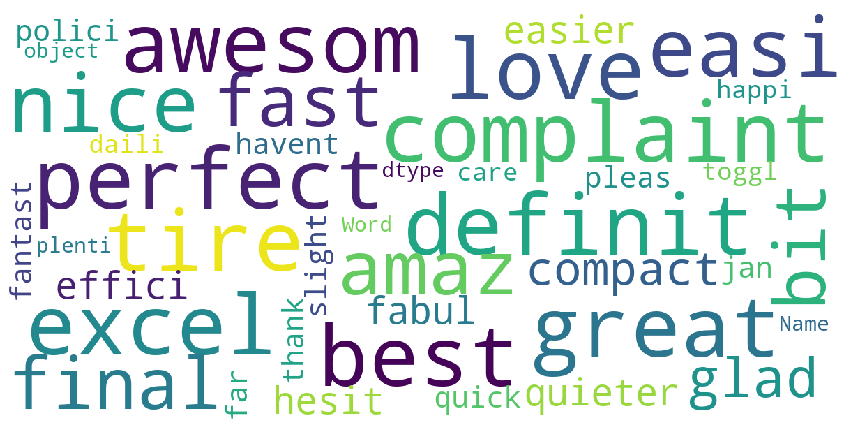
\includegraphics[height=7cm,width=14cm]{por.png}}
	\caption{Certain descriptors of quality are evidently bound up withs specific ratings.}
	\label{fig2}
\end{figure}
Figure.~\ref{fig2}~ shows the association strength between each word of the reviews and its corresponding rating. It can be intuitively expressed as the bigger the word, the stronger the association. The detail of result can be checked in appendix.1 
\subsubsection{Sentimental rating}
The attitude of the review $R$ to the product can be expressed in Sentimental Rating $E$, which can be formulated as
\begin{gather}
 E_{i}=\sum_{n=1} ^{N}e_{n}, e_{n}\in R
\end{gather}
where $N$ denotes the length of the review $R$. $e_{n}$ is the coefficients of each word in the review $R$. ????????


\begin{table}[H]
	\centering
	\caption{Sentimental rating measure for each review}	
	\setstretch{1}  %设置表的行间距
	\begin{tabular}{cc}
		\toprule[1.5pt]
		\multicolumn{1}{m{4cm}}{\centering Review id} & \multicolumn{1}{m{5cm}}{\centering Sentimental rating} \\
		\midrule[1pt]
		R1SO9VMCIGZX3U     	 & 24.020178\\
		R2E7N0TVLUHUDR     & -11.512384 \\
		R1A3ZUBR8TSAKY          &8.748561\\
		$\cdots$     &	$\cdots$ \\
		RLJNYBK4FGBYX          &17.712887\\
		R26QCW75C4JDOK          &4.191633\\
		\bottomrule[1.5pt]
	\end{tabular}\label{Rating}
\end{table}


\section{Time-based Reputation Model}
Due to result of Sentimental Analysis that some reviews might show attitude deviating from their star rating, we draw up the credibility of the reviews and ratings. Thus, the model can reflect the change of products' reputation reliably.
\subsection{Review Credibility}
The credibility $C$ is defined to reflect the effective information contained in the reviews and ratings. It can be simply formulated below 
\begin{gather}
C=\frac{h}{t} (t\neq 0)
\end{gather}
where $h$ denotes the amount of voters that vote the review as helpful and $t$ represents the total of voters. As we assume all the reviews with $t=0$ have the $C$ equal to $0$, the relation matrix of $C$ and star rating of the database of baby pacifier can be give as below 
%为了找出最有帮助的评论,我们可以通过helpful\_votes,total\_votes进行建模。以奶嘴为例子,做出Upvote = helpful\_votes除以total\_votes的分箱后关系矩阵,如图\ref{llssll}所示
\begin{figure}[H]
\centering
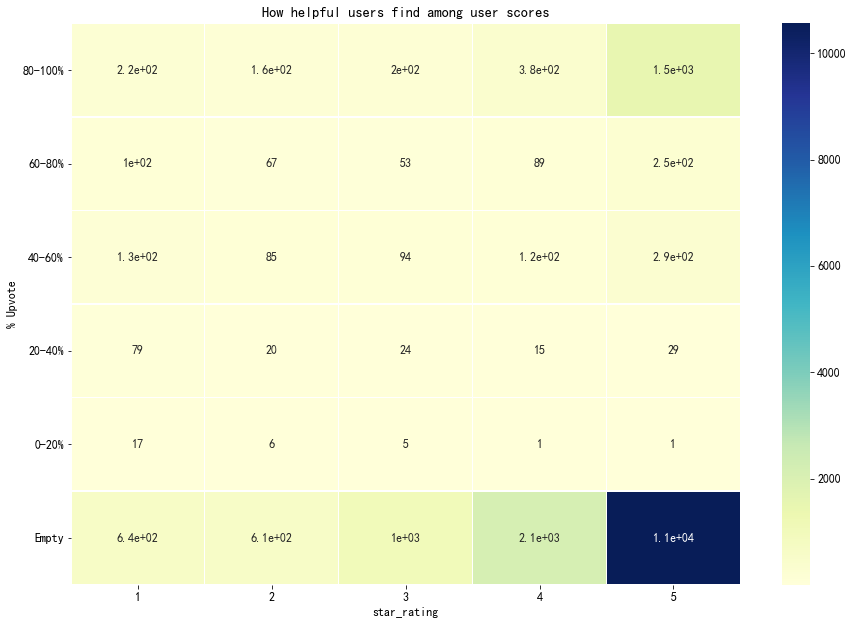
\includegraphics[width=\textwidth]{Upvote.png}%.4代表宽度大小正常为1

\caption{The relationship between score and voting}\label{llssll}%caption里面是题目,label为标签,\ref引用
\end{figure}
The elements in the matrix is the quantity of corresponding reviews. It can be analysised that 
\begin{itemize} 
	\item  [\textbf{a}.] Most of the reviewers are inclined to give a high rating.
	\item  [\textbf{b}.] More than half of the reviews have no vote, especially the recent ones.
\end{itemize}
%可以看出,
%* Reviews are skewed towards positive
%* More than half of the reviews are with zero votes.大部分的评论都没有点赞,特别是一些最新的评论
%* Many people agree with score 5 reviews(大V一般都是正面的,很多人追随他们好评)
We would utilize the LightGBM algorithm to recompute the credibility $C$ for all reviews in following stage. Thus, we could gain the exact credibility of all reviews even the non-vote ones that are too new to be noticed.

\subsection{LightGBM Recomputing}
The LightGBM\cite{lgb,lgb2} model shows high performance in processing the features with different measure\footnote{\quad For example, the length of review and whether the reviewer is a vine are both feature of the review but have different meature.}. We take a part of early reviews as training set and output the credibility of later reviews.

%由于各个指标(比如大v,词向量,rating,verified\_purchase等)的量纲不同,传统方法(如上文提到的Logistic回归只是用来区分词向量的好坏)对Upvote进行预测有一定的局限性,而决策树模型可以很好的避免量纲带来的问题,我们采取的是目前最新的Lightgbm\cite{lgb}进行决策并计算出Helpfulness(Upvote)。

\begin{figure}[H]
	\centering
	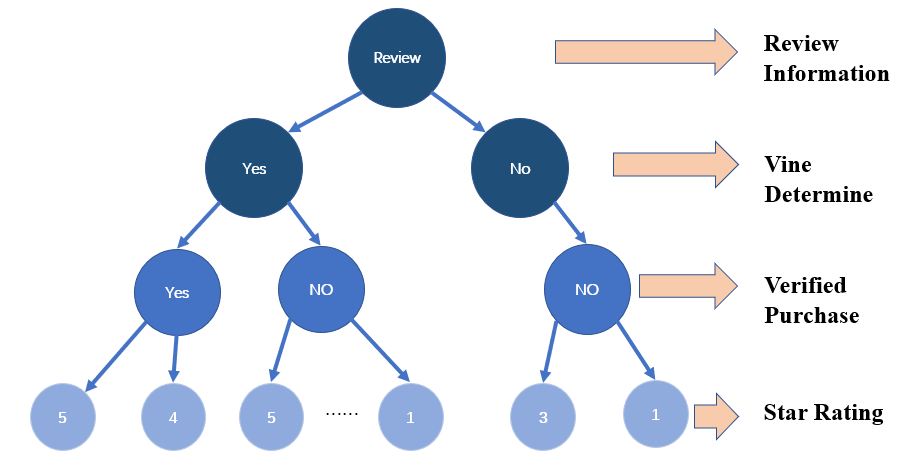
\includegraphics[width=\textwidth]{shu.png}%.4代表宽度大小正常为1
	\caption{Schematic diagram of various features decided by LightGBM.}\label{llsaall}%caption里面是题目,label为标签,\ref引用
\end{figure}

通过\ref{llsaall}所示的决策树模型,we can 计算出 the credibility $C$ in the table \ref{biassssoss} as 

\begin{table}[H]
	\centering
	\caption{Credibility of microwave ovens' review}	
	\setstretch{1.3}  %设置表的行间距
	\begin{tabular}{ccccc}
		\toprule[1.5pt]
		\multicolumn{1}{m{3.5cm}}{\centering Review id} & \multicolumn{1}{m{2cm}}{\centering Star rating}&
		\multicolumn{1}{m{1cm}}{\centering Vine}&
		\multicolumn{1}{m{3cm}}{\centering Date}&
		\multicolumn{1}{m{2.5cm}}{\centering \textbf{Credibility}}\\
		\midrule[1pt]
		R3HT7OGKQO8Q0E &5&Y&2010-11-22&0.762627\\
		R3LXL05NPDK7P2 &5&N	&2010-11-23	&0.566363\\
		RWZZ77PTTHCDV &4&Y&2010-11-28&0.928533\\
		R2JK82HHMUGGOU &1&N&2010-12-21&0.089120\\
		$\cdots $&$\cdots $&$\cdots $&$\cdots $&$\cdots $\\
		RJ4HTF6UC3JGC &2&N&2015-08-22&0.240850\\
		R1X47WDNBT4OHZ &1&N&2015-08-23&0.843194\\
		R9T1FE2ZX2X04 &5&Y&2015-08-31&0.710421\\
		\bottomrule[1.6pt]
	\end{tabular}\label{biassssoss}
\end{table}

由表 \ref{biassssoss}所示,一般大V的高分评论的可信度都很好,一方面也说明了大v的影响力;而像一些普通用户会因为一些不当的言论,被别人打差评,导致那些评论的可信程度不是太高。

%\subsection{Net promoter score}
%As a gauge that represents how the enterprise and employees treat customers, NPS(Net Promoters Score) signals the possibility that users recommend products and services to their colleagues and friends. In this sense, customers are classified as recommenders, passives and detractors. NPS helps us evaluate customer satisfaction and loyalty\cite{nsp}. NPS is defined as
%NPS(Net Promoters Score) 是现有用户向其他人推荐你的产品和服务的可能性指数。是一种用来测量企业及员工如何对待客户的度量指标。在这一度量内,客户被划分为三大种类:推荐者、被动者和贬损者。也就是客户是否愿意将公司或产品推荐给朋友或同事。通过NPS helps us evaluate customer satisfaction and loyalty\cite{nsp}, 其计算方式如下:
%\begin{gather}
%NPS = (Promoters - Detractors)/Total ratings * 100
%\end{gather}
%Where the reviews with rating 1,2 are regarded as Detractors while the ones with Rating 3 and Rating 4,5 are Passive and Promoters respectly.



\subsection{Reputation model}
Before showing the fluctuation of the products' reputation, we draw up the model to quantify reputation of the product in a fixed time period $\Delta T$,which can be give as
\begin{gather}
P=\frac{\sum_{n=1}^{N}R \cdot H}{\sum_{n=1}^{N} H}
\end{gather}
where the $P$ reflect the reputation during the time slot $\Delta T$, in which the amount of updated reviews equal to $N$. $H$ is the weight for each review, which can be yeilded as 
\begin{gather}
H=\left\{\begin{matrix}C ,(V=0)
\\ 10C,(V=1)
\end{matrix}\right.
\end{gather}
where $C$ denote the help-rating, and the index $V$ denoted whether the reviewer is a vine. The $V$ equal to $1$ when the reviewer is a vine or $0$ when not. We input the database of several most-review products to yeild the result as follows 
\begin{figure}[H]
	\centering
	\subfigure[product 1]{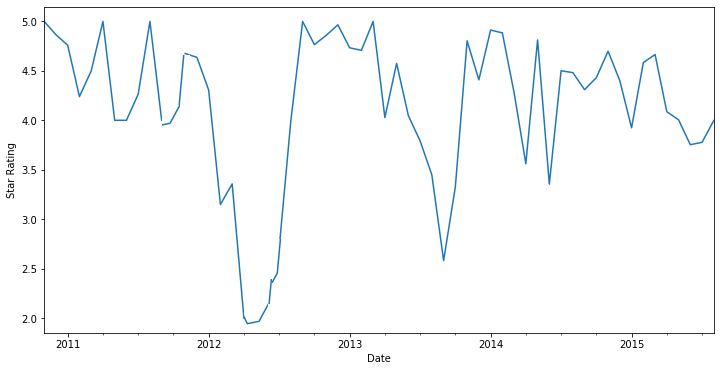
\includegraphics[height=4cm,width=7cm]{./pic/p1.png}}
	\subfigure[product 2]{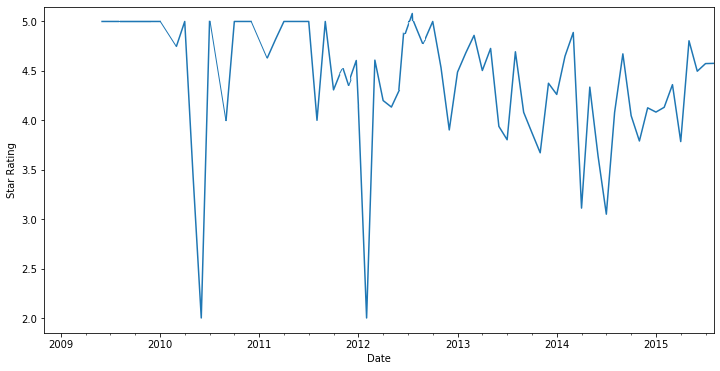
\includegraphics[height=4cm,width=7cm]{./pic/p20.png}}
	
	\centering
	\subfigure[product 3]{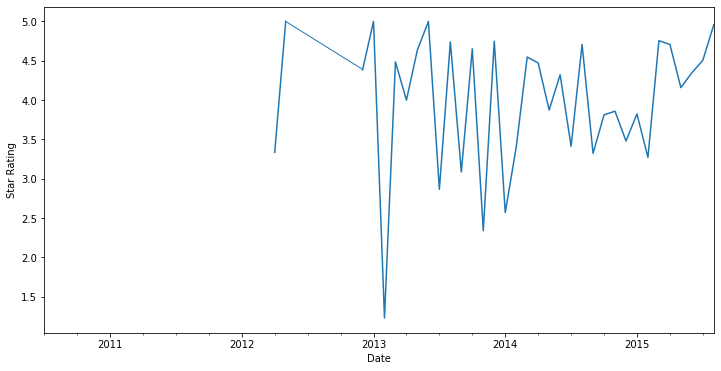
\includegraphics[height=4cm,width=7cm]{./pic/p30.png}}
	\subfigure[product 4]{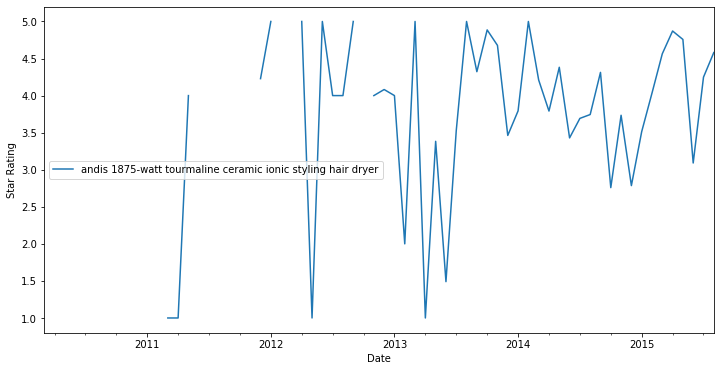
\includegraphics[height=4cm,width=7cm]{./pic/p4.png}}
	\caption{Product reputation chart over time.}\label{repu}	
\end{figure}
The figure~\ref{repu}~ shows that the product-2 has a more stable than the other products while the product-1 has the most dramatic changes druing the period. Product-3 and product-4 are new to the market and have large fluctuations. One can gain the reputation fluctuation of any products by take their databases into the time-based model.
The detail result can be checked in appendix \ref{d}.


%%%%%%%%%%%%%%%%%%%%%%%%%%%%%%%模型建立%%%%%%%%%%%%%%%%%%%%%%%%%%%%%%%%%%%%%%
\section{Combinations of Text and Rating}

\subsection{Association Rule Analysis}
\subsection{Support and Confidence}
A review can be rewritten as item sets $I=\left \{  i_{1},i_{2},\cdots,i_{m}\right \}$, where the element $i$ represents the word contained in the corresponding review. Thus, the superset of all reviews can be given as item data base $D=\left \{ I \right \}$. The amount of elements of item set is defined as the length of item set, so that the $k-length$ item set $I$ can be rewritten as $I_{k}$. For any two item sets $X\subseteq I_{x}$ and $Y\subseteq I_{y}\quad(x,y\in \left \{ 1,2,\cdots,n \right \})$ , the Support of $X$ and $Y$ can be defined as 
\begin{gather}
Sup(X\bigcap Y)=\frac{num(X\bigcap Y)}{num(AllSample)}
\end{gather}
where the $num(X\bigcap Y)$ and $num(AllSample)$ denotes the amount of reviews containing both $X$ and $Y$ and the quantity of all reviews respectively. The $X\bigcap Y$ can be regarded as the frequent item sets(FIS)\cite{bib:4} when $Sup(X,Y)>Sup_{min}$ ,  where the  $Sup_{min}$ is the minimum Support threshold. The Confidence of $X$ to $Y$ can be given as 
\begin{gather}
Conf(X\leftarrow Y)=\frac{num(XY)}{num(Y)}
\end{gather}
 The FIS $X$ and $Y$ will be deemed as strongly associated\cite{bib:4} if $Conf(X\leftarrow Y)>Conf_{min}$, where $Conf_{min}$ is the minimum Confidence threshold.
\subsection{Apriori algorithm}
The algorithm is used to find out all the FIS. Obviously,when the word sets $X$ is FIS,
its subsets are all FIS\cite{bib:66}, which can be fomulated as 
\begin{gather}
Sup(X)\geqslant Sup(X\bigcap Y)>Sup_{min}
\end{gather}
Moreover the supersets of $X$ will be all non-FIS if the $X$ is non-FIS\cite{bib:66}, which can be represent as
\begin{gather}
Sup_{min}>Sup(X)\geqslant Sup(X\bigcap Y)
\end{gather}
Thus, we could gain the process of Apriori algorithm based on this two feature 
, the pseudocode in appendix \ref{ee}.
 
%\begin{algorithm}[H]
%	\caption{Procedure of Apriori}  
%	\LinesNumbered  
%	\setstretch{1}   %设置表的行间距
%	\KwIn{item data base: $D$\newline
%		 minimum Support threshold: $Sup_{min}$\newline
%		 minimum Confidence threshold: $Conf_{min}$
%	}
%	\KwOut{frequent item sets $F$}  
%\textbf{Initialize} \newline
%iteration $t\leftarrow 1$ \newline
% The candidate FIS:$C_{t}=\varnothing$ \newline
% The length of FIS:$length=1$ \newline
%       \For{i=1 to sizeof(D)}
%        {$I_{i}$=D(i)\newline
%        	n=sizeof($I_{i}$)\newline
%         \For{j=1 to n}{
%         \If{$I_{i}(j)\notin C_{t}$ }
%         {$C_{t}=C_{t}\cup I_{i}(j) $}
%     }
%   }
%            $F_{t}=\left \{ f|f\in C_{t},Sup(f)>Sup_{min}\right \}$\newline
%     \While{$F\neq \varnothing$}
%     { t=t+1\newline 
%     	length=length+1\newline	
%     	$C_{t}\leftarrow $ all candidate of FIS in $F_{t-1}$\newline
%      $F_{t}=\left \{ f|f\in C_{t},(Sup(f)>Sup_{min})\bigcap (Comf(f)>Conf_{min}) \right\}$\newline
%     }	
%	\Return{$F_{t-1}$} 
%\end{algorithm} 
We input the database of microwave oven to yeild the result showed in table~\ref{sssfff}~. The table ??? shows the frequent item sets including the highest or the lowest star ratings and their corresponding words combinations. We sum up the coefficient of the word showed in table ~\ref{biasssssso}~ in each combination to gain the text-based measures. Due to the measures combinations the successful product can be regarded as having a average rating-based measures not less than ??? and text-based measures not less than ???, while the failing one have the rating-based measures not more than ??? and text-based measures not more than ???.

\begin{table}[H]
	\centering
	\caption{????????????????????}	
	\setstretch{1.3}  %设置表的行间距
	\begin{tabular}{c|ccc}
		\toprule[1.5pt]
		\multicolumn{1}{m{2cm}}{\centering Label} &
		\multicolumn{1}{m{6cm}}{\centering Words set} & \multicolumn{1}{m{2cm}}{\centering Star rating}&
		\multicolumn{1}{m{2cm}}{\centering  Sentimental Rating}\\
		\midrule[1pt]
		&$\big [$ quiet, new, small, compact $\big ]$ &5&7.16581\\
			successful	&$\big [$ practic, much, pleasant, good $\big ]$ &5&6.24621\\
				 	&$\cdots$ $\cdots$&$\cdots$&$\cdots$\\
	 	&$\big [$ good, great, nice $\big ]$ &5&5.84687\\
				\midrule[1pt]
		&$\big [$prong, needless, unmanag$\big ]$ &1&-4.81354\\
						 	&$\cdots$ $\cdots$&$\cdots$&$\cdots$\\
	failing	&$\big [$ open, total, wast, locat $\big ]$ &1&-5.18134\\
				&$\big [$ loud, bad, wrong, old , damag $\big ]$ &1&-6.47152\\
		\bottomrule[1.6pt]
	\end{tabular}\label{sssfff}
\end{table}



\section{Dynamic Time Warping}
The star rating and sentimental score of each pruduct can be transform into time series as $A=[a_{1},a_{2},\cdots,a_{s}]$ and $B=[b_{1},b_{2},\cdots,b_{s}]$ where  $a_{i}$ and $b_{i}$  represent the average rating during $t_{i}$ to $t_{i+1}$. The point in time $\left \{ t_{i}  \right \}$ differ by a constant $\Delta t$, which can be expressed as $t_{i+1}-t_{i}=\Delta t$. 
For the time series $A$ and $B$ have different dimensions, we would execute dimensionless processing as follows
\begin{gather*}
a_{i}\leftarrow a_{i}/a_{max}\\
b_{i}\leftarrow b_{i}/b_{max}
\end{gather*}
Where $a_{max}$ and $b_{max}$ denote the maximum of star rating and sentimental score. Moreover, we remove $\left \{b_{1},\cdots,b_{m}\right \}(1\leqslant m<s)$ from $B$ to identify the specific star ratings would incite more reviews with the similar sentiment in subsequent period, so that the time series $B$ can be rewritten as $B=[b_{1},b_{2},\cdots,b_{t}] (t<s)$. The distance between $a_{i}$ and $b_{j}$ can be given as $\delta(a_{i},b_{j})$. Thus, the correlation between reviews and star rating can be given as
\begin{gather}
 D=\frac{\sum_{n=1}^{N}\delta(a_{i},b_{j})\cdot W_{n}}{\sum_{n=1}^{N}W_{n}}
\end{gather}
where $D$ is the weighted average of the distance between time series $A$ and $B$, which has negative correlation with the relevance between the star rating and future reviews. After setting all the weights as 1, the minimum of $D$ can be calculated in the algorithm as follow%或许需要补充说明

\begin{algorithm}[H]
	\caption{Procedure of DWT}  
	\LinesNumbered  
	\setstretch{1}   %设置表的行间距
	\KwIn{Rating time series: $A=[a_{1},a_{2},\cdots,a_{s}]$\newline
		  Review time series: $B=[b_{1},b_{2},\cdots,b_{t}]$
	}
	\KwOut{Series correlation D} 
	\textbf{Let} $\delta$ be a distance between coordinates of sequence \newline
    \textbf{Let} m(S,T) be the matrix of couples(cost,path)\newline
   $ m[1,1,1:2]\leftarrow(\delta(a,b),(0,0)) $\newline
    \For{i=2 to s}{
    $ m[i,1,1:2]\leftarrow(m[i,1,1]+\delta(a_{i},b_{1}),(i-1,1)) $
}
     \For{j=2 to T}{
	$ m[1,j,1:2]\leftarrow(m[1,j-1,1]+\delta(a_{1},b_{j}),(1,j-1)) $
   }
 \For{i=2 to s}{
    \For{j=2 to T}{
    $minimum\leftarrow minVal(m[i-1,j,1],m[i,j-1,1],m[i-1,j-1,1])$\newline
    $m[i,j,1:2]\leftarrow(first(minimum)+\delta(a_{i},b_{j}),second(minimum))$
}
}
	\Return{$ M[S,T]$} 
\end{algorithm} 
We input the data of \text{Danby 0.7 cu.ft. countertop microwave} into the algorithm to yeild an example wraping path in figure.~\ref{FFFF}~. The figure.~\ref{FFFF}~ shows that the wraping degree is slight, which means that the text-based measures reflect strong similarity with previous star ratings. Thus, it can be deemed that the specific star ratings incite more corresponding reviews.
\begin{figure}[H]
	\centering
	\subfigure[time series of rating]{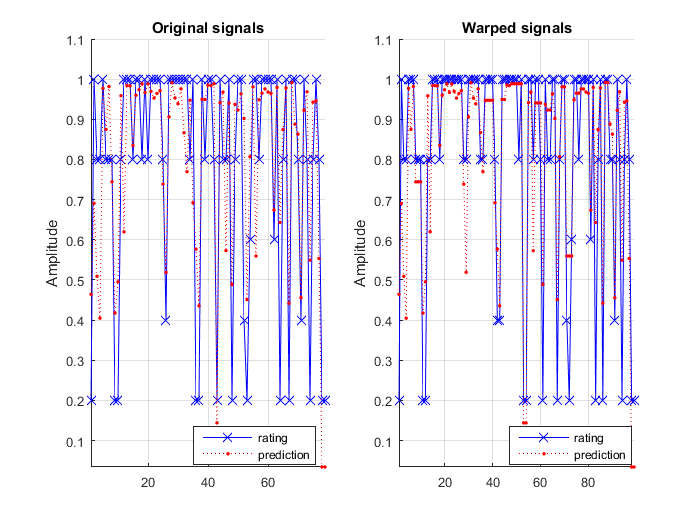
\includegraphics[height=7cm,width=7cm]{dtw_p.png}}
	\subfigure[wraping path]{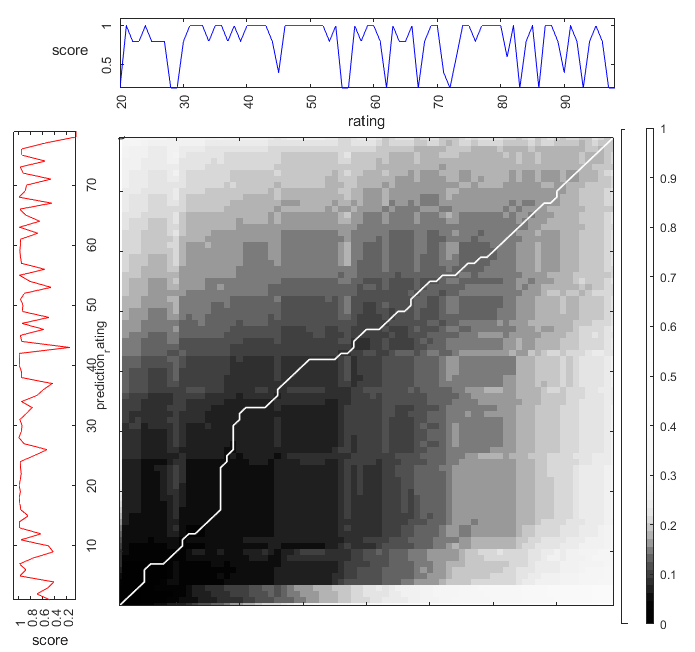
\includegraphics[height=7cm,width=7cm]{dtw.png}}
	\caption{ Result yeilded by DWT.}
	\label{FFFF}
\end{figure}
After identifying the specific star ratings incite more corresponding reviews, we compare the inciting rate within the pruduct with the most reviews in table.~\ref{biasssso}~. It can be discovered that star ratings of the pacifier are more likely to incite corresponding reviews.
\begin{table}[H]
	\centering
	\caption{Inciting rate of the best-sell product.}	
	\setstretch{1.3}  %设置表的行间距
	\begin{tabular}{c|cc}
		\toprule[1.5pt]
		\multicolumn{1}{m{2cm}}{\centering Product} &
		\multicolumn{1}{m{9cm}}{\centering Product title} & \multicolumn{1}{m{2cm}}{\centering Distance}\\
		\midrule[1pt]
		&andis 1875-watt fold-n-go ionic hair dryer &1.0255098\\
		hair dryer&remington salon collection pearl ceramic hair dryer     & 1.0337255\\
		&conair 1875 watt tourmaline ceramic hair dryer          &1.0421478\\
		\midrule[1pt]
		&danby 0.7 cu.ft. countertop microwave          & 0.6733481\\
		microwave&whirlpool wmc20005yw  countertop microwave          &0.82484716\\
		&sharp microwave drawer oven        &0.8349739\\
				\midrule[1pt]
		&philips avent bpa free contemporary freeflow pacifier        &1.403347\\
		pacifier&philips avent bpa free soothie pacifier       &1.086339\\
		&wubbanub infant pacifier - giraffe&1.101904\\
		\bottomrule[1.6pt]
	\end{tabular}\label{biasssso}
\end{table}


%%%%%%%%%%%%%%%%%%%%%%%%%%%%%%%灵敏度分析%%%%%%%%%%%%%%%%%%%%%%%%%%%%%%%%%%%
\section{Sensitivity Analysis}

%在进行词向量的编码处理时,我们对Word2Vec和TF-IDF进行过参数的调整,从而使得到的词向量能很准确的区分消极的和积极的评论。下面我们对比一些参数对二分类的影响,并利用可视化技术进行观察,得到结果如下:
We select proper parameters of Word2Vec and TF-IDF to precisely discriminate positive and negative reviews. Then we compare the difference of some parameters on bigram and visualize the results as shown above.

\begin{figure}[H]
	\centering
	\subfigure[TF-IDF with default parameters ]{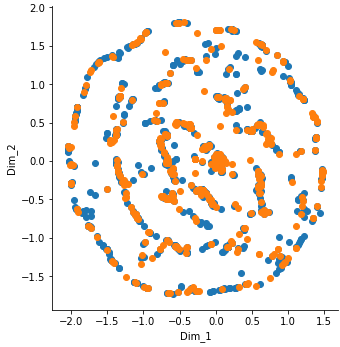
\includegraphics[height=6cm,width=7cm]{11.png}}
	\subfigure[TF-IDF with perplexity:10, iter:1500]{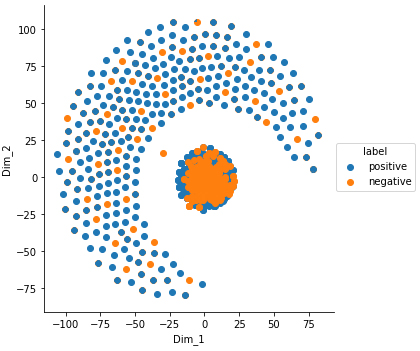
\includegraphics[height=6cm,width=7cm]{2.png}}

	
		\centering
	\subfigure[Word2Vec with default parameters ]{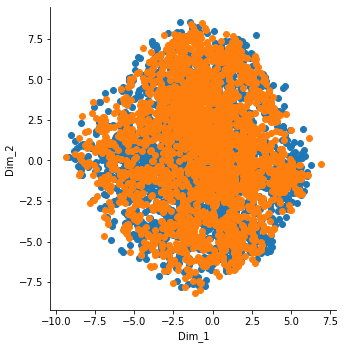
\includegraphics[height=6cm,width=7cm]{13.png}}
	\subfigure[Word2Vec with perplexity:20, iter:2000 ]{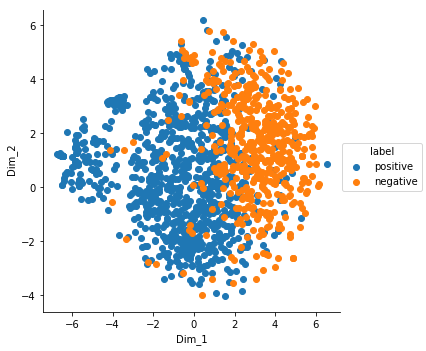
\includegraphics[height=6cm,width=7cm]{12.png}}
	\caption{Visualization of word vectors under different parameters.}
	\label{fisg}
\end{figure}

It is obvious from the figure that the high-dimensional words vector after adjustment has a good distinguishing plane, and the Logistics Regression we adopt in the dichotomy training takes salient effect.
%从图中很明显可以看出,我们调参之后的高维词向量具有很好的区分平面,在二分类训练任务中,我们采取的Logistics Regression将会有不错的效果。

In task e, we only adopt adjective words. When adding all key words (e.g. add nouns in operation), the accuracy of analyzing the effect of specific quality descriptors on text-based measures can not be guaranteed. In a specific two-star rating example, we notice that some of those significant coefficients are not meaningful, e.g. 'junk'. However, after conducting cleaning, they manifest qualities as shown in Figure ~\ref{fissssg}~.
%In task e, we only adopt adjective words. When adding all key words(e.g. add nouns in operation), the accuracy can 
%在任务e中,我们仅仅采用的是adjective words。 当用所有的关键词句(比如名词等也加进去)后,由于有像微波炉这样的词语,并不能很准确的分析出不同星级对specific quality descriptors of text-based,我们以二星为例可以注意到 notice that some of those significant coefficients are not meaningful, e.g. 'junk'.,而在我们清理后能非常明显表现出quality like this:


\begin{figure}[H]
	\centering
	\subfigure[Before cleaning word vector and part of speech ]{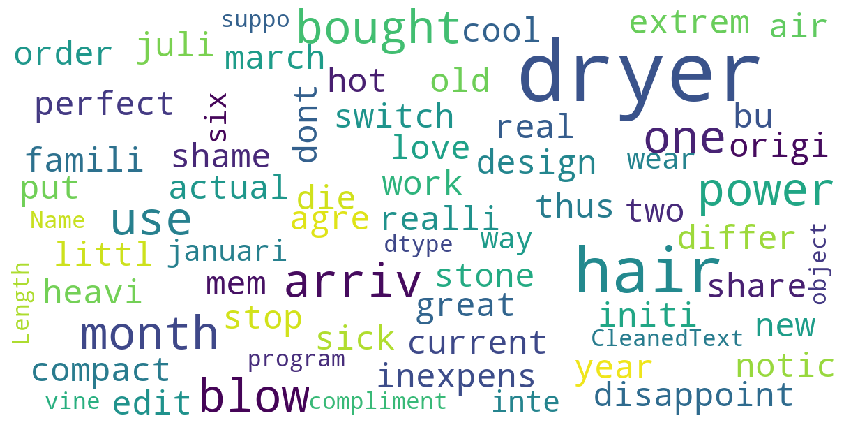
\includegraphics[height=6cm,width=7cm]{cfj2.png}}
	\subfigure[After cleaning word vector and part of speech ]{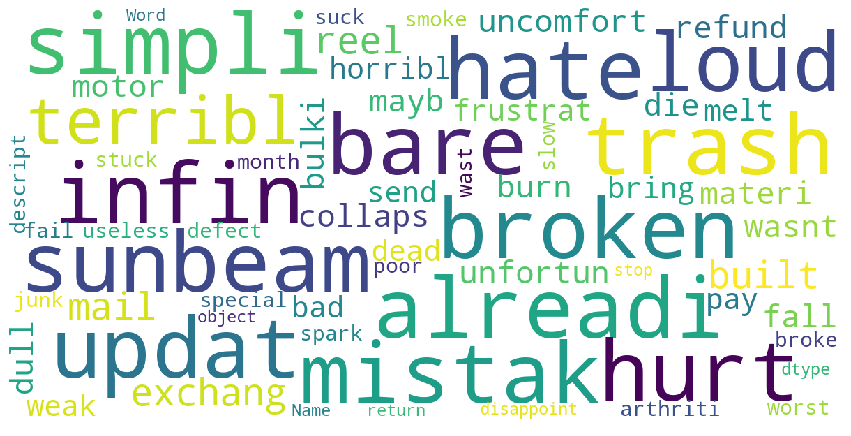
\includegraphics[height=6cm,width=7cm]{cfj22.png}}
	\caption{???}
	\label{fissssg}
\end{figure}






%%%%%%%%%%%%%%%%%%%%%%%%%%%%%%%优缺点%%%%%%%%%%%%%%%%%%%%%%%%%%%%%%%%%%%
\section{Strength and Weaknesses}
\subsection{Strength}
\begin{itemize}
	\item \textbf{Compatibleness.} Combining models in text analysis, we see good agreement and robustness in three given products.%Due to the model combination adopted in text analysis, the robustness is so great that the model can adjust to reviews of totally different products. 
	\item \textbf{Efficiency.} Owing to the Gradient Boosting Decision Tree algorithm adopted in ???????????, the data with differet dimensions can be processed smoothly and efficiently.
	\item \textbf{Parameters.} Most of our models are non-parametric, and our parametric models guarantee
	the convergence. Hence, there is no need to worry too much about the parameters.
\end{itemize}

\subsection{Weaknesses}
\begin{enumerate}
	\item 
	
	%没有考虑纸飞机在不同受力情况下的形变,将纸飞机视作了刚体,和实际情况有较大差别。
	
\end{enumerate}

%%%%%%%%%%%%%%%%%%%%%%%%%%%%%%%展望%%%%%%%%%%%%%%%%%%%%%%%%%%%%%%%%%%%
\section{Conclusions and Discussion}
We propose three major models by effectively combining reviews and ratings. Our models exhibit great potential in drawing conclusions as following:

\begin{itemize}
	\item We introduce Sentiment Prediction model, the result of which is a direct and positive answer to the connection question, that is, certain descriptors of quality are indeed evidently connected with rating levels. 
	\item In response to inquiry on internal relationship between ratings and reviews, Dynamic Time Warp model, our second model, compares the similarities of ratings and sentimental scores. Through the best warping path, we find that specific ratings incite more corresponding reviews. 
	\item (This item requires rethinking!) In terms of time-based measures and patterns, we establish Temporal Critical Assessment model to determine the most informative data measures for Sunshine Company to track. These data measures are:.(The content is reserved for discussion)
	\item  By introducing Net Promoter Score and feeding it to time-based procedure, we manage to draw a map that symbolizes the period-rating map. On this foundation, we offer our suggestions to facilitate online activities concerning three commodities.
	\item  The final list of combination of selected instructions and appropriate recommendations is determined by a two-step selection algorithm (This requires rethinking!). 
\end{itemize}

	
%%%%%%%%%%%%%%%%%%%%%%%%%%%%%%%参考文献%%%%%%%%%%%%%%%%%%%%%%%%%%%%%%%%%%%
\newpage
\setmainfont{Times New Roman}
\fancyhf{}
%\fancyhead[R]{ }
\fancyhead[L]{Team \footnotesize{\#} 2015970}
\nocite{*}		
\begin{thebibliography}{9}
	\bibitem{bib:1}Herlocker, J. L., Konstan, J. A., Terveen, L. G., and Riedl, J. T., Evaluating Collaborative Filtering Recommender Systems. ACM Trans. on Information Systems, 22, 1, 2004, 5-53.
	\bibitem{bib:2}Mudambi S M, Schuff D. Research note: What makes a helpful online review? A study of customer reviews on Amazon. com[J]. MIS quarterly, 2010: 185-200.
	\bibitem{amsu}Cheng Z, Ding Y, Zhu L, et al. Aspect-aware latent factor model: Rating prediction with ratings and reviews[C]//Proceedings of the 2018 world wide web conference. 2018: 639-648.
	\bibitem{232}Park S, Nicolau J L. Asymmetric effects of online consumer reviews[J]. Annals of Tourism Research, 2015, 50: 67-83.
	\bibitem{233} Danescu-Niculescu-Mizil, C., Kossinets, G., Kleinberg, J., $\&$ Lee, L. (2009).
	Tourism Research, 50, 67–83
	 \bibitem{234}Kokkodis M. Learning from positive and unlabeled Amazon reviews: Towards identifying trustworthy reviewers[C]//Proceedings of the 21st International Conference on World Wide Web. 2012: 545-546.
	\bibitem{236}Leino, J., $\&$ Räihä, K.-J. (2007). Case amazon. Proceedings of the 2007 ACM Conference on Recommender Systems - RecSys ’07.
	\bibitem{BOW}Wallach H M. Topic modeling: beyond bag-of-words[C]//Proceedings of the 23rd international conference on Machine learning. 2006: 977-984.
	\bibitem{BOW2}Zhang Y, Jin R, Zhou Z H. Understanding bag-of-words model: a statistical framework[J]. International Journal of Machine Learning and Cybernetics, 2010, 1(1-4): 43-52.
	\bibitem{TF}Ramos J. Using tf-idf to determine word relevance in document queries[C]//Proceedings of the first instructional conference on machine learning. 2003, 242: 133-142.
	\bibitem{word}Rong X. word2vec parameter learning explained[J]. arXiv preprint arXiv:1411.2738, 2014.
	\bibitem{word2}Goldberg Y, Levy O. word2vec Explained: deriving Mikolov et al.'s negative-sampling word-embedding method[J]. arXiv preprint arXiv:1402.3722, 2014.
	\bibitem{word3}Lilleberg J, Zhu Y, Zhang Y. Support vector machines and word2vec for text classification with semantic features[C]//2015 IEEE 14th International Conference on Cognitive Informatics \& Cognitive Computing (ICCI* CC). IEEE, 2015: 136-140.
	\bibitem{t}Linderman G C, Rachh M, Hoskins J G, et al. Efficient algorithms for t-distributed stochastic neighborhood embedding[J]. arXiv preprint arXiv:1712.09005, 2017.
	\bibitem{lg}Hosmer Jr D W, Lemeshow S, Sturdivant R X. Applied logistic regression[M]. John Wiley \& Sons, 2013.
	\bibitem{bbb}Juneja P, Ojha U. Casting online votes: to predict offline results using sentiment analysis by machine learning classifiers[C]//2017 8th International Conference on Computing, Communication and Networking Technologies (ICCCNT). IEEE, 2017: 1-6.
	\bibitem{lgb}Ke G, Meng Q, Finley T, et al. Lightgbm: A highly efficient gradient boosting decision tree[C]//Advances in neural information processing systems. 2017: 3146-3154.
	\bibitem{lgb2}Prokhorenkova L, Gusev G, Vorobev A, et al. CatBoost: unbiased boosting with categorical features[C]//Advances in neural information processing systems. 2018: 6638-6648.
	\bibitem{nsp}Grisaffe D B. Questions about the ultimate question: conceptual considerations in evaluating Reichheld's net promoter score (NPS)[J]. Journal of Consumer Satisfaction, Dissatisfaction and Complaining Behavior, 2007, 20: 36.
	\bibitem{bib:4}Ye Y, Chiang C C. A parallel apriori algorithm for frequent itemsets mining[C]//Fourth International Conference on Software Engineering Research, Management and Applications (SERA'06). IEEE, 2006: 87-94.
	\bibitem{bib:66}Lenca P, Vaillant B, Meyer P, et al. Association rule interestingness measures: Experimental and theoretical studies[M]//Quality Measures in Data Mining. Springer, Berlin, Heidelberg, 2007: 51-76.
	
\end{thebibliography}


%%%%%%%%%%%%%%%%%%%%%%%%%%%%%%%附录%%%%%%%%%%%%%%%%%%%%%%%%%%%%%%%%%%%
\newpage
\appendix
\section*{Appendices}\addcontentsline{toc}{section}{Appendices for Data and Code}\label{Appendices}

\fontsize{13pt}{12.5pt}\selectfont
Here is \textbf{Code and Figures} we used in our paper, which python is the main development language. Since we mainly use \textbf{jupyter notebook} for programming, most of the python code will only be represented by pictures in the appendix. Some important model code will be placed here. The detailed working code can be found on ours gitHub repository\footnote{\quad https://github.com/2015970/MCMICM2020}.
\vspace{7pt}
\textbf{\subsection*{Appendices A : Exploratory Data Analysis in the paper}\label{a}}
\begin {figure}[h]
\centering % 居中显示

\includegraphics[width=7cm,height=4cm]{protect.jpg}
\caption{Mapping description of the relationship between Amazon reviews and users via Visio.} % 标题
\end {figure}

\begin{figure}[H]
	\centering
	\subfigure[The relationship between score and voting. ]{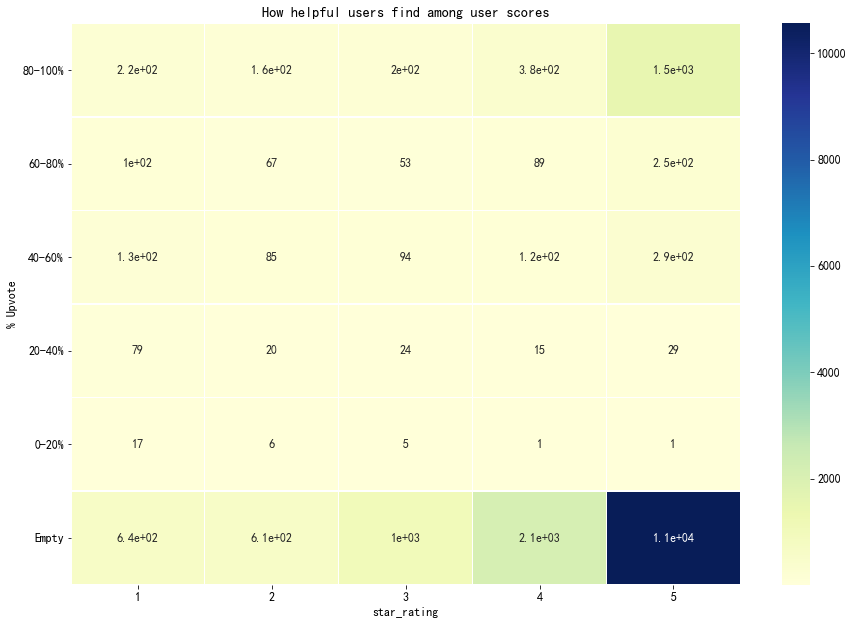
\includegraphics[height=4cm,width=7cm]{Upvote.png}}
	\subfigure[The 'star\_rating' with the distribution of 'vine'	]{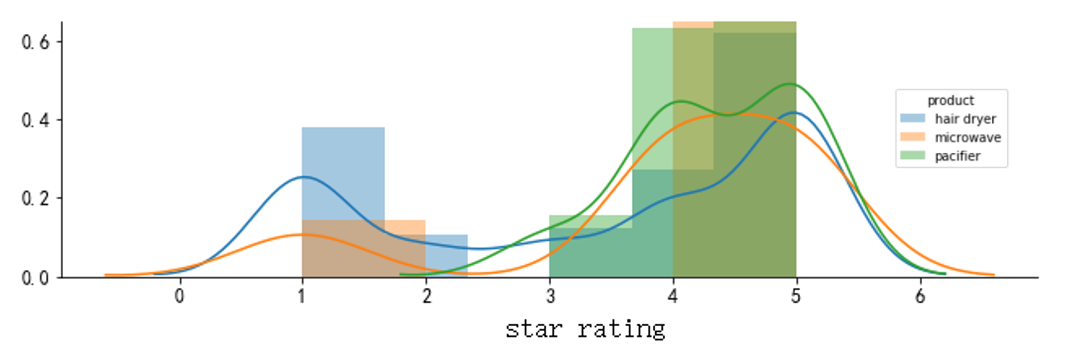
\includegraphics[height=4cm,width=7cm]{score.png}}
	\caption{Exploratory Data Analysis.}
\end{figure}

\textbf{\textcolor[rgb]{0.98,0.00,0.00}{Exploratory Data Analysis}}
\lstinputlisting[language={python},numbers=left,numberstyle=\tiny,
rulesepcolor=\color{red!20!green!20!blue!20},  
keywordstyle=\color{blue!70!black},  
commentstyle=\color{blue!90!},  
basicstyle=\ttfamily] {./code/text.py}

\textbf{\subsection*{Appendices B : Text processing and sentiment analysis for question 1, 2-a and 2-e}\label{b}}

\begin{figure}[H]
	\centering
	\subfigure[TF-IDF with default parameters ]{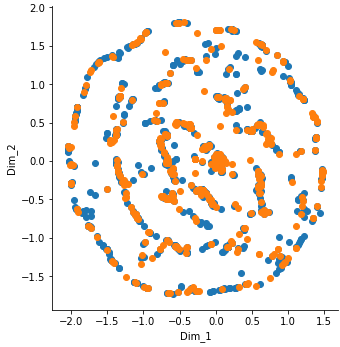
\includegraphics[height=4cm,width=6cm]{11.png}}
	\subfigure[TF-IDF with perplexity:10, iter:1500]{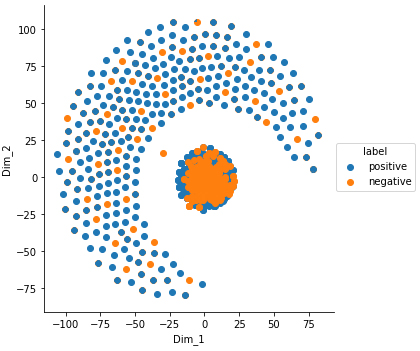
\includegraphics[height=4cm,width=6cm]{2.png}}
	
	\centering
	\subfigure[Word2Vec with default parameters ]{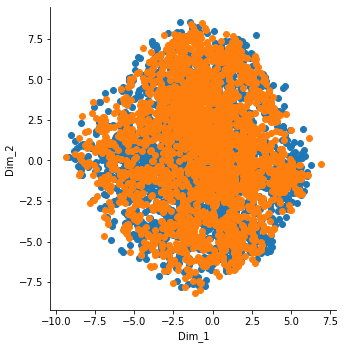
\includegraphics[height=4cm,width=6cm]{13.png}}
	\subfigure[Word2Vec with perplexity:20, iter:2000 ]{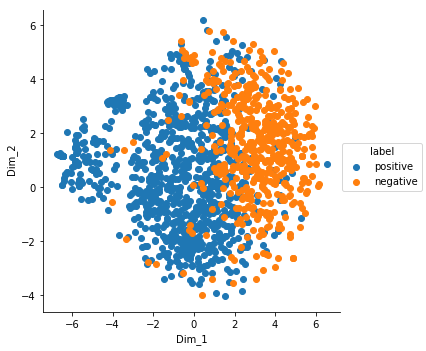
\includegraphics[height=4cm,width=6cm]{12.png}}
	\caption{Visualization of word vectors under different parameters.}
\end{figure}

\begin{figure}[H]
	\centering
	\subfigure[Pacifier's positive reviews]{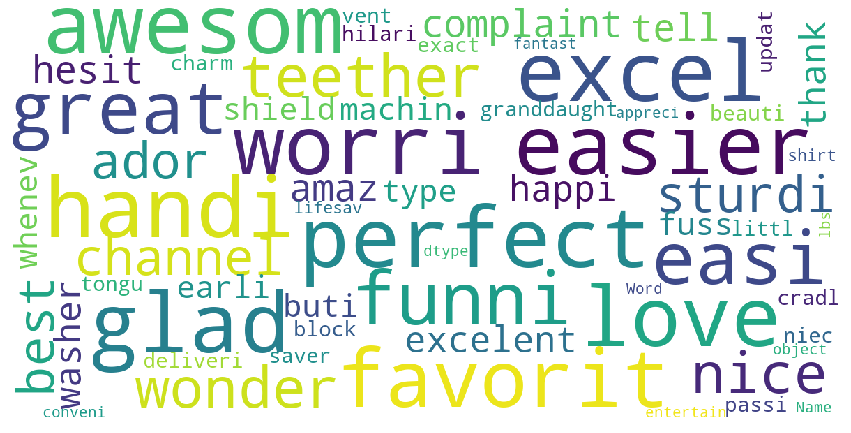
\includegraphics[height=4cm,width=7cm]{./pic/demo/11.png}}
	\subfigure[Pacifier's negative reviews]{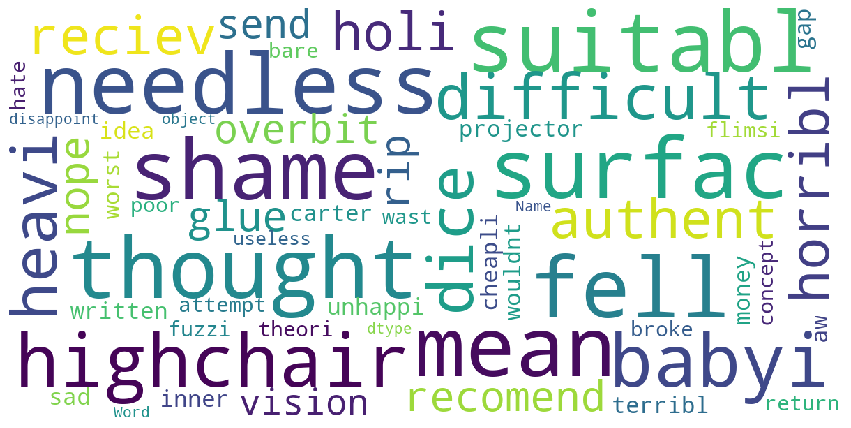
\includegraphics[height=4cm,width=7cm]{./pic/demo/1.png}}
	
	\centering
	\subfigure[Hair dryer's positive reviews]{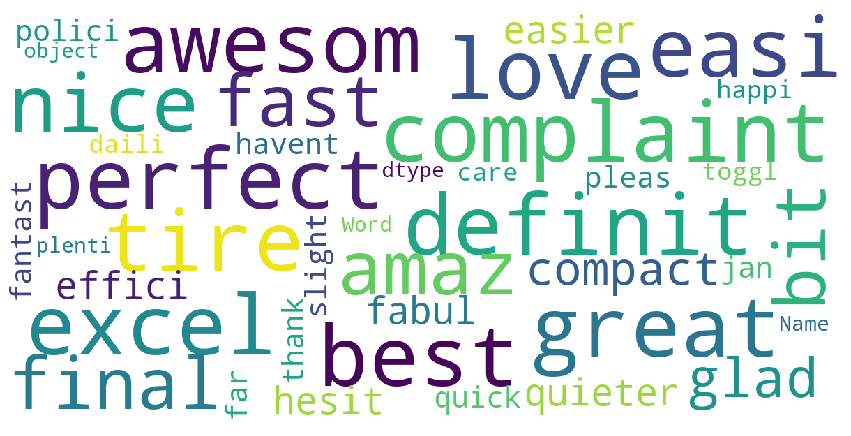
\includegraphics[height=4cm,width=7cm]{./pic/demo/22.png}}
	\subfigure[Hair dryer's negative reviews]{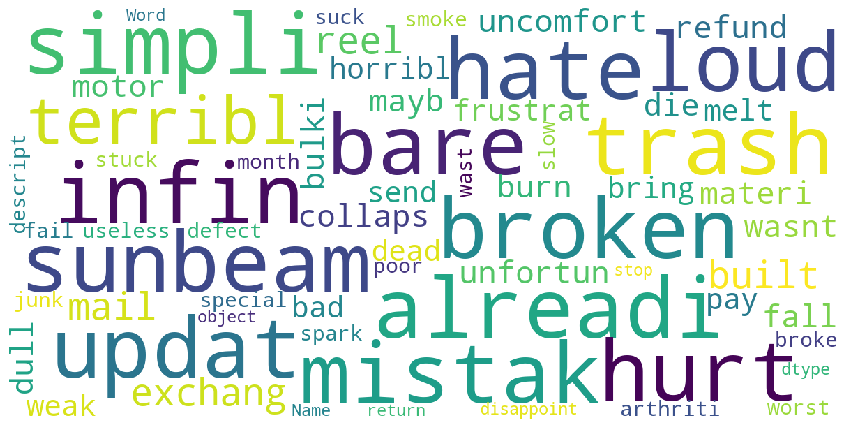
\includegraphics[height=4cm,width=7cm]{./pic/demo/2.png}}
	
	\centering
	\subfigure[Microwave's positive reviews]{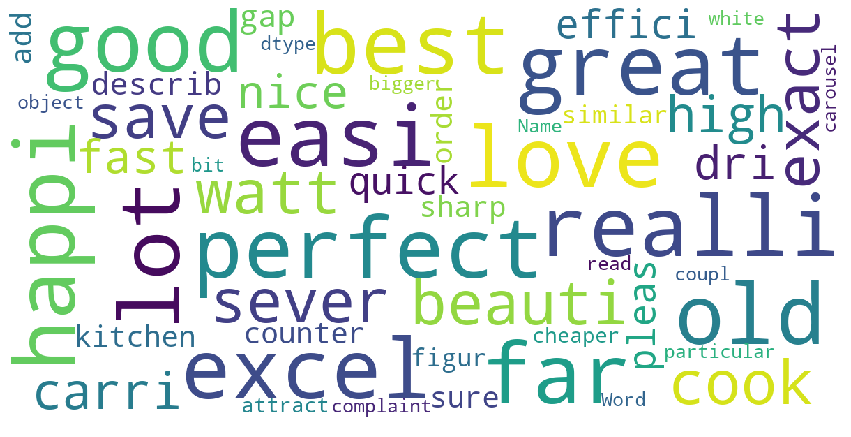
\includegraphics[height=4cm,width=7cm]{./pic/demo/33.png}}
	\subfigure[Microwave's negative reviews]{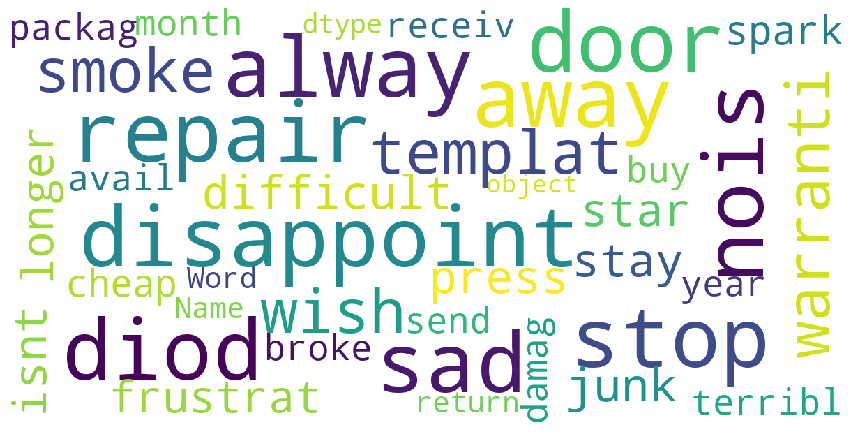
\includegraphics[height=4cm,width=7cm]{./pic/demo/3.png}}
\end{figure}

\textbf{\textcolor[rgb]{0.98,0.00,0.00}{Text processing main code via python}}
\lstinputlisting[language={python},numbers=left,numberstyle=\tiny,
rulesepcolor=\color{red!20!green!20!blue!20},  
keywordstyle=\color{blue!70!black},  
commentstyle=\color{blue!90!},  
basicstyle=\ttfamily] {./code/text2.py}

\textbf{\textcolor[rgb]{0.98,0.00,0.00}{Logistic Regression main code}}
\lstinputlisting[language={python},numbers=left,numberstyle=\tiny,
rulesepcolor=\color{red!20!green!20!blue!20},  
keywordstyle=\color{blue!70!black},  
commentstyle=\color{blue!90!},  
basicstyle=\ttfamily] {./code/text3.py}

\textbf{\subsection*{Appendices C : Dynamic Time Warping mian code for question 2-d}\label{c}}
\begin{figure}[H]
	\subfigure[time series of rating]{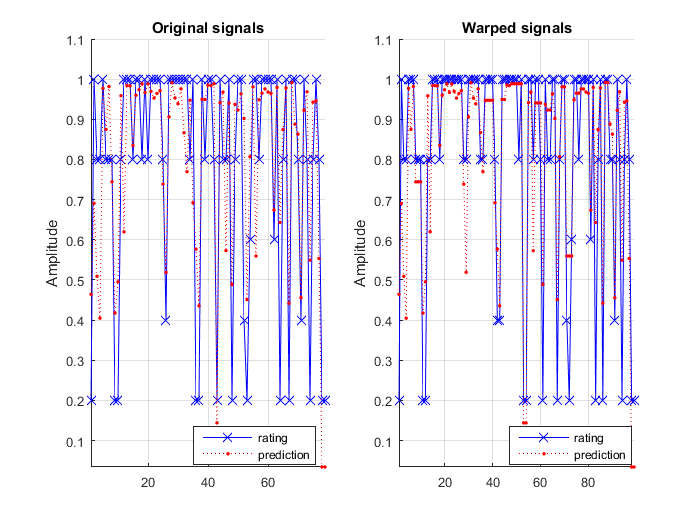
\includegraphics[height=7cm,width=7cm]{dtw_p.png}}
	\subfigure[wraping path]{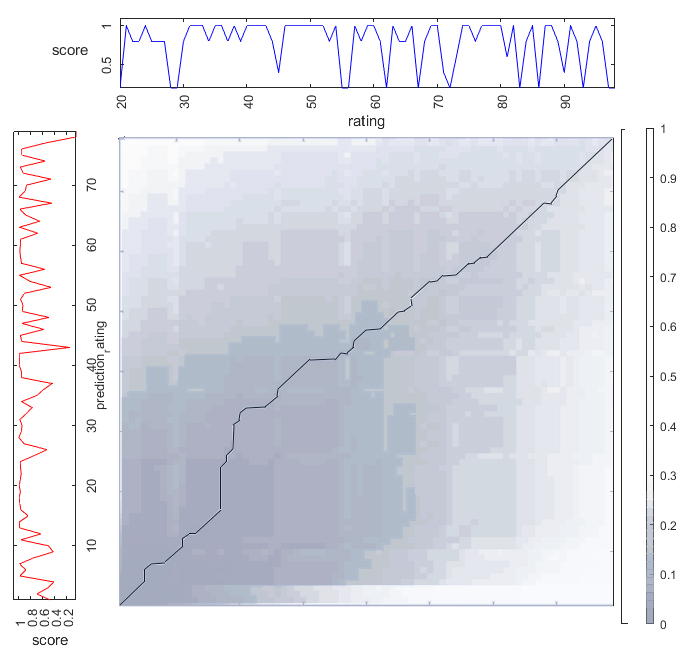
\includegraphics[height=7cm,width=7cm]{dtw2.jpg}}
	\caption{ Result yeilded by DWT.}
\end{figure}

\textbf{\textcolor[rgb]{0.98,0.00,0.00}{Dynamic Time Warping main code via matlab (The drawing code is too long and omitted)}}
\lstinputlisting[language={matlab},numbers=left,numberstyle=\tiny,
rulesepcolor=\color{red!20!green!20!blue!20},  
keywordstyle=\color{blue!70!black},  
commentstyle=\color{blue!90!},  
basicstyle=\ttfamily] {./code/dtw.m}

\begin{table}[H]
	\centering
	\caption{Inciting rate of the best-sell product.}	
	\setstretch{1.3}  %设置表的行间距
	\begin{tabular}{c|cc}
		\toprule[1.5pt]
		\multicolumn{1}{m{2cm}}{\centering Product} &
		\multicolumn{1}{m{9cm}}{\centering Product title} & \multicolumn{1}{m{2cm}}{\centering Distance}\\
		\midrule[1pt]
		&andis 1875-watt fold-n-go ionic hair dryer &1.0255098\\
		hair dryer&remington salon collection pearl ceramic hair dryer     & 1.0337255\\
		&conair 1875 watt tourmaline ceramic hair dryer          &1.0421478\\
		\midrule[1pt]
		&danby 0.7 cu.ft. countertop microwave          & 0.6733481\\
		microwave&whirlpool wmc20005yw  countertop microwave          &0.82484716\\
		&sharp microwave drawer oven        &0.8349739\\
		\midrule[1pt]
		&philips avent bpa free contemporary freeflow pacifier        &1.403347\\
		pacifier&philips avent bpa free soothie pacifier       &1.086339\\
		&wubbanub infant pacifier - giraffe&1.101904\\
		\bottomrule[1.6pt]
	\end{tabular}
\end{table}

\textbf{\subsection*{Appendices D : Temporal Reputaion and information for 2-a, 2-b}\label{d}}
\begin{figure}[H]
	\centering
	\subfigure[product 1]{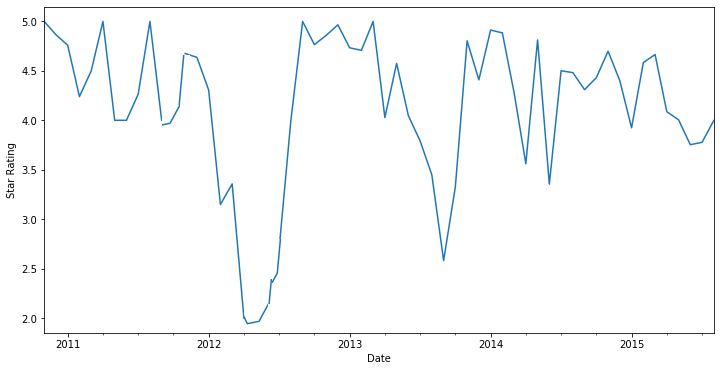
\includegraphics[height=4cm,width=7cm]{./pic/p1.png}}
	\subfigure[product 2]{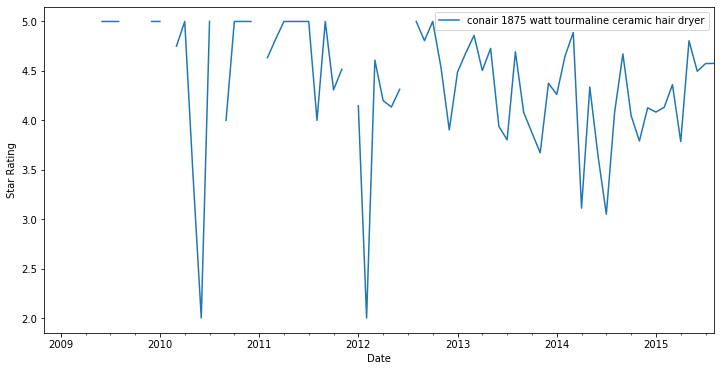
\includegraphics[height=4cm,width=7cm]{./pic/p2.png}}
	
	\centering
	\subfigure[product 3]{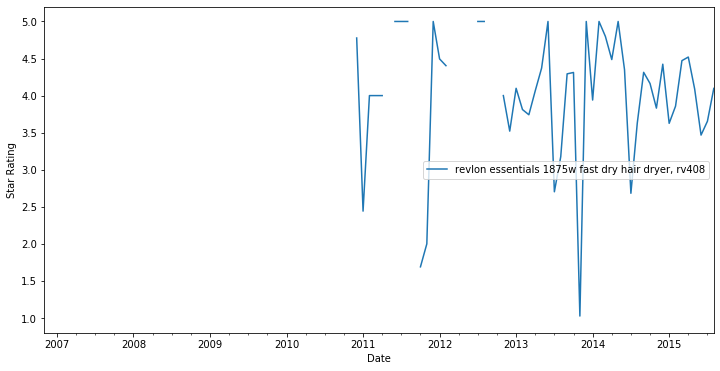
\includegraphics[height=4cm,width=7cm]{./pic/p3.png}}
	\subfigure[product 4]{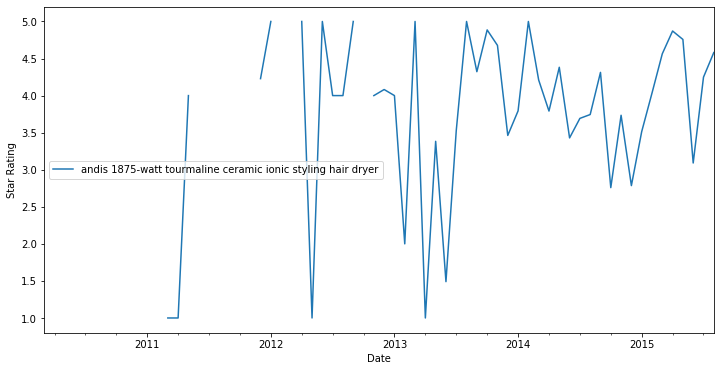
\includegraphics[height=4cm,width=7cm]{./pic/p4.png}}
	\caption{Product reputation chart over time.}	
\end{figure}

\textbf{\textcolor[rgb]{0.98,0.00,0.00}{text-based measure(s) and ratings-based measures.}}
\lstinputlisting[language={python},numbers=left,numberstyle=\tiny,
rulesepcolor=\color{red!20!green!20!blue!20},  
keywordstyle=\color{blue!70!black},  
commentstyle=\color{blue!90!},  
basicstyle=\ttfamily] {./code/time.py}

\begin{table}[H]
	\centering
	\caption{LightGBM calculated importance(credibility)}	
	\setstretch{1.3}  %设置表的行间距
	\begin{tabular}{ccccc}
		\toprule[1.5pt]
		\multicolumn{1}{m{3.5cm}}{\centering Review id} & \multicolumn{1}{m{2cm}}{\centering Star rating}&
		\multicolumn{1}{m{1cm}}{\centering Vine}&
		\multicolumn{1}{m{3cm}}{\centering Date}&
		\multicolumn{1}{m{2.5cm}}{\centering \textbf{credibility}}\\
		\midrule[1pt]
		R3HT7OGKQO8Q0E &5&Y&2010-11-22&0.762627\\
		R3LXL05NPDK7P2 &5&N	&2010-11-23	&0.566363\\
		RWZZ77PTTHCDV &4&Y&2010-11-28&0.928533\\
		R2JK82HHMUGGOU &1&N&2010-12-21&0.089120\\
		$\cdots $&$\cdots $&$\cdots $&$\cdots $&$\cdots $\\
		RJ4HTF6UC3JGC &2&N&2015-08-22&0.240850\\
		R1X47WDNBT4OHZ &1&N&2015-08-23&0.843194\\
		R9T1FE2ZX2X04 &5&Y&2015-08-31&0.710421\\
		\bottomrule[1.6pt]
	\end{tabular}\label{biassssossss}
\end{table}

\textbf{\subsection*{Appendices E : Apriori algorithm 2-c}\label{ee}}
\textbf{\textcolor[rgb]{0.98,0.00,0.00}{Because the code is too long, it is represented by pseudo code}}

\begin{algorithm}[H]
	\caption{Procedure of Apriori}  
	\LinesNumbered  
	\setstretch{1}   %设置表的行间距
	\KwIn{item data base: $D$\newline
		minimum Support threshold: $Sup_{min}$\newline
		minimum Confidence threshold: $Conf_{min}$
	}
	\KwOut{frequent item sets $F$}  
	\textbf{Initialize} \newline
	iteration $t\leftarrow 1$ \newline
	The candidate FIS:$C_{t}=\varnothing$ \newline
	The length of FIS:$length=1$ \newline
	\For{i=1 to sizeof(D)}
	{$I_{i}$=D(i)\newline
		n=sizeof($I_{i}$)\newline
		\For{j=1 to n}{
			\If{$I_{i}(j)\notin C_{t}$ }
			{$C_{t}=C_{t}\cup I_{i}(j) $}
		}
	}
	$F_{t}=\left \{ f|f\in C_{t},Sup(f)>Sup_{min}\right \}$\newline
	\While{$F\neq \varnothing$}
	{ t=t+1\newline 
		length=length+1\newline	
		$C_{t}\leftarrow $ all candidate of FIS in $F_{t-1}$\newline
		$F_{t}=\left \{ f|f\in C_{t},(Sup(f)>Sup_{min})\bigcap (Comf(f)>Conf_{min}) \right\}$\newline
	}	
	\Return{$F_{t-1}$} 
\end{algorithm} 
\begin{table}[H]
	\centering
	\caption{Best indicate a potentially successful or failing product.	}	
	\setstretch{1}  %设置表的行间距
	\begin{tabular}{c|ccc}
		\toprule[1.5pt]
		\multicolumn{1}{m{2cm}}{\centering Sentimental} &
		\multicolumn{1}{m{6cm}}{\centering Words set} & \multicolumn{1}{m{2cm}}{\centering Star rating}&
		\multicolumn{1}{m{2cm}}{\centering  Coefficient}\\
		\midrule[1pt]
		&$\big [$ quiet, new, small, compact $\big ]$ &5&7.16581\\
		successful	&$\big [$ practic, much, pleasant, good $\big ]$ &5&6.24621\\
		&$\big [$ good, great, nice $\big ]$ &5&5.84687\\
		\midrule[1pt]
		&$\big [$prong, needless, unmanag$\big ]$ &1&-4.81354\\
		failing	&$\big [$ open, total, wast, locat $\big ]$ &1&-5.18134\\
		&$\big [$ loud, bad, wrong, old , damag $\big ]$ &1&-6.47152\\
		\bottomrule[1.6pt]
	\end{tabular}
\end{table}


\end{document}

